	\documentclass[10pt,oneside]{CBFT_book}
	
	% Algunos paquetes
	
	\usepackage{amssymb}
	\usepackage{amsmath}
	\usepackage{graphicx}
	\usepackage{libertine}
	\usepackage{lipsum}
	\usepackage[numbers]{natbib}
% 	\usepackage{natbib}
	\setcitestyle{square}

	\usepackage{polyglossia}
	\setdefaultlanguage{spanish}


	\usepackage{CBFT.estilo} % Cargo la hoja de estilo

	% Tipografías
	% \setromanfont[Mapping=tex-text]{Linux Libertine O}
	% \setsansfont[Mapping=tex-text]{DejaVu Sans}
	% \setmonofont[Mapping=tex-text]{DejaVu Sans Mono}

	%===================================================================
	%	DOCUMENTO PROPIAMENTE DICHO
	%===================================================================

% \title{CBFT Mecánica clásica}
% \author{Simetrías}
% \date{\today}

\begin{document}
% \maketitle
% \tableofcontents
\chapter{Simetrías}

% =================================================================================================
\section{Constantes de movimiento y simetrías}
% =================================================================================================

Si en las ecuaciones de Euler-Lagrange
\[
	\frac{d}{dt}\left( \dpar{\Lag}{\dot{q}_j} \right) - \dpar{\Lag}{q_j}  = 0, 
\]
se daba el caso de que $ \Lag $ no dependía de $ q_j $ entonces
$ \partial {\Lag} /\partial {q_j}  = 0  $ y
\[
	\frac{d}{dt}\left( \dpar{\Lag}{\dot{q}_j} \right) = 0
\]
significa que 
\[
	\dpar{\Lag}{\dot{q}_j} \equiv p_j
\]
es una constante ($\dot{p}_j=0$).

Por otra parte, si $\delta q_i$ es traslación rígida en una dirección $\hat{n}$ entonces 
\[
	p_i = \vb{P}\cdot\hat{n} \qquad \text{ y } \qquad Q_j= \vb{F}\cdot\hat{n}. 
\]	
En cambio, si $\delta q_i$ es una rotación rígida en torno a un eje $\hat{n}$ se tiene 
\[
p_i = \vb{L}\cdot\hat{n} \qquad  \text{ y } \qquad Q_j= \vb{\Tau}\cdot\hat{n}.
\]

En estos dos casos
\[
	\dpar{T}{q_i} = 0
\]
puesto que:
\begin{itemize}
 \item Como $T$ depende de las velocidades (y no de las coordenadas) no depende del origen y por lo tanto no 
varía ante una traslación rígida (que es un cambio de origen).
 \item Como $T$ es un escalar no cambia ante una rotación.
\end{itemize}

% \[
% 	\dpar{\Lag}{q_i} = 0 = \dpar{T}{q_i} - \dpar{V}{q_i} = 0
% \]
Luego, si $V \neq V(\dot{q})$ (el potencial $V$ no depende explícitamente de las velocidades) entonces las ecuaciones 
de Euler-Lagrange adoptan la forma
% \[
% 	\frac{d}{dt}\left( \dpar{T}{\dot{q}_j} \right) + \dpar{V}{q_j}  = 0 
% \]
\[
	\frac{d}{dt}\left( \dpar{T}{\dot{q}_j} \right) = - \dpar{V}{q_j}   
\]
\[
	\frac{d}{dt}\left( p_j \right) = - \dpar{V}{q_j}   
\]
y entonces 
\[
	\dot{p}_j = -\dpar{V}{q_j}   
\]
es la fuerza total proyectada en la dirección $\hat{n}$.

\notamargen{Acá parecen estar separadas los movimientos rígidos del hecho de que V sea de las coordenadas solamente. 
En un caso tenemos $\dot{p}=0$ y en otro $\dot{p} = -\partial V / \partial q$.
Creo que lo del potencial sería para las otras coordenadas no afectadas por la simetría?.}

Para examinar constantes de movimiento podemos ver primero las variables cíclicas. Sin embargo, si elegimos otras 
coordenadas tal vez no aparezca la constante de movimiento como coordenada cíclica (aunque por supuesto sigue 
existiendo dicha constante).

\subsection{Simetrías en el lagrangiano}

Sea un cambio de coordenadas $q_i \to q_i'$, si como resultado de éste se tenía
\[
	\Lag(q_i, \dot{q}_i, t ) = \Lag(q_i(q_i',t), \dot{q}_i(\dot{q}_i',t), t ),
\]
es decir, que al escribir el lagrangiano en función de las nuevas coordenadas obtengo el mismo, se está ante la 
presencia de una simetría asociada.

Las variables cíclicas son un caso particular de teorema de Noether. Una transformación infinitesimal genérica de $k$ 
grados de libertad es
\begin{eqnarray*}
	q'_1 &= q_1 + \varepsilon g_1(q_1,...,q_k,t) \\
	q'_2 &= q_2 + \varepsilon g_2(q_1,...,q_k,t) \\
	... \\
	q'_k &= q_k + \varepsilon g_k(q_1,...,q_k,t)
\end{eqnarray*}

Para una traslación infinitesimal rígida se tiene 
\begin{eqnarray*}
	x'_i = x_i + \delta x \\
	y'_i = y_i + \delta y \\
	z'_i = z_i + \delta z
\end{eqnarray*}
o bien $\vb{x}' = \vb{x} + \delta \vb{x}$ y la energía cinética 
\[
	T = \sum_i \frac{1}{2} m_i v_i^2
\]
es invariable puesto que depende de las velocidades (que no dependen del origen) y se da $\dot{x} = \dot{x}'$ y lo 
mismo para las otras coordenadas.

Para una rotación en el plano $xy$
\begin{eqnarray*}
	x'_i = x_i + \varepsilon y_i \\
	y'_i = y_i - \varepsilon x_i \\
	z'_i = z_i 
\end{eqnarray*}
que matricialmente se pueden ver como 
\[
	\begin{pmatrix}
	x_i'\\
	y_i'
	\end{pmatrix}
	=
	\begin{pmatrix}
	 1 & \varepsilon \\
	 -\varepsilon & 1
	\end{pmatrix}
	\begin{pmatrix}
	 x_i \\
	 y_i
	\end{pmatrix}
	\qquad 
	\begin{pmatrix}
	 1 & -\varepsilon \\
	 \varepsilon & 1
	\end{pmatrix}
	\begin{pmatrix}
	\dot{x}_i'\\
	\dot{y}_i'
	\end{pmatrix}
	=
	\begin{pmatrix}
	\dot{x}_i \\
	\dot{y}_i
	\end{pmatrix}
\]
resulta
\[
	T = \sum_i \frac{1}{2} m_i v_i^2 = \frac{1}{2} \sum_i m_i ( \dot{x}_i^2 + \dot{y}_i^2 )
\]
y ahora para $T'$ expresamos las coordendas primitivas en función de las nuevas (primadas).
\[
	T' = \frac{1}{2} \sum_i m_i ( [\dot{x}_i' - \varepsilon \dot{y}_i' ]^2 + [\dot{y}_i' + \varepsilon 
\dot{x}_i']^2 )
\]
y a primer orden
\[
	T' = \frac{1}{2} \sum_i m_i ( \dot{x}^{'2}_i - 2 \varepsilon \dot{y}_i'\dot{x}_i' + 
 	2 \varepsilon \dot{y}_i'\dot{x}_i' + \dot{y}^{'2}_i ) = 
 	\frac{1}{2} \sum_i m_i( \dot{x}^{'2}_i + \dot{y}^{'2}_i ) = T.
\]
\notamargen{Resolver un problema de double superscript aquí. T es invariante porque es básicamente un escalar.}

Entonces $T$ es invariante ante traslación rígida y rotación rígida.
Faltaría completar este análisis con las simetrías del potencial $V$ para ver las simetrías del lagrangiano.
En los casos en que 
\[
	V = V(|\vb{x}_i - \vb{x}_j|) \quad \text{ Invariancia de traslación en cualquier dirección} 
\]
lo cual significa depender de la distancia relativa. Otro caso es:
\[
	V = V( x_i, y_i ) \quad \text{ Invariancia de traslación en $z$}
\]

Noether dice que si el lagrangiano $\Lag$ es invariante entonces hay una simetría de la transformación que no 
necesariamente es rotación rígida o traslación rígida.
\[
	T \text{ se conserva en } \begin{cases}
	                           \text{ rotación rígida } \\
	                           \text{ traslaciones }
	                          \end{cases}
\]
\[
	V \text{ tendrá } \begin{cases}
			   \text{ 1. rotación rígida } \\
			    \text{ 2. traslación } \\
			     \text{ 3. rotación y traslación } \\
	                  \end{cases}
\]

Luego, digamos que:
\begin{itemize}
 \item $\Lag$ tiene un momento lineal si $V$ tiene 1
 \item $\Lag$ tiene un momento angular si $V$ tiene 2 
 \item $\Lag$ tiene una combinación de momento lineal y angular si $V$ tiene 3
\end{itemize}

Si se tiene constante de movimiento, no necesariamente el lagrangiano $\Lag$ tiene esa simetría.

Una trasnformación general para $k$ grados de libertad se escribe como 
\begin{eqnarray*}
	q'_1 &= q_1 + \sum_{\ell=1}^S \varepsilon_\ell g_1^\ell(q_1,...,q_k,t) \\
	q'_2 &= q_2 + \sum_{\ell=1}^S \varepsilon_\ell g_2^\ell(q_1,...,q_k,t) \\
	... \\
	q'_k &= q_k + \sum_{\ell=1}^S \varepsilon_\ell g_k^\ell(q_1,...,q_k,t)
\end{eqnarray*}
donde el término en cada sumatoria corresponde al $\delta q_k$.

\notamargen{La simetría de paridad $\vb{x}\to -\vb{x}$, que es una reflexión tiene la particularidad de que es 
discreta, no se puede ir continuamente.}

\subsection{Rotación en 3D infinitesimal}






% =================================================================================================
\section{El teorema de Noether}\index{Noether, teorema de}
% =================================================================================================

Si existe una transformación continua $q_i \longrightarrow q_i + \delta q_i$ que deje invariante el
$\Lag$ entonces hay una constante de movimiento asociada a dicha transformación.

La transformación se puede escribir 
\[
	q_i \longrightarrow q_i' = q_i + \delta q_i
\]
y cumple 
\[
	\Lag(q_i, \dot{q}_i , t) = \Lag(q_i', \dot{q}_i' , t) =
	\Lag(q_i[q_i',t], \dot{q}_i[\dot{q}_i',t] , t)
\]
y así si consideramos una variación a $t$ fijo, también vale que 
\[
	\delta \Lag = \sum_i \dpar{\Lag}{q_i}\delta q_i + \dpar{\Lag}{\dot{q}_i}\delta \dot{q}_i =
	\sum_i \dpar{\Lag}{q_i}\delta q_i + \frac{d}{dt}\left( \dpar{\Lag}{\dot{q}_i}\delta q_i \right)
	- \frac{d}{dt}\left( \dpar{\Lag}{\dot{q}_i} \right) \delta q_i = 0
\]
\[
	\delta \Lag = \sum_i \left[ \dpar{\Lag}{q_i} - \frac{d}{dt}\left( \dpar{\Lag}{\dot{q}_i} \right) \right]
	\delta q_i + \frac{d}{dt}\left( \dpar{\Lag}{\dot{q}_i}\delta q_i \right) = 0
\]
pero como el primer término del RHS es nulo por las ecuaciones de Euler-Lagrange tenemos que 
\[
	\delta \Lag = \frac{d}{dt}\left( \sum_i \dpar{\Lag}{\dot{q}_i}\delta q_i \right)  = 0,
\]
lo que está dentro del paréntesis es la cantidad conservada. 

Existe una simetría (que deja invariante al lagrangiano) y resulta en una constante de movimiento.
No obstante, no toda constante de movimiento proviene de una simetría.

% ~~~~~~~~~~~~~~~~~~~~~~~~~~~~~~~~~~~~~~~~~~~~~~~~~~~~~~~~~~~~~~~~~~~~~~
\begin{ejemplo}{\bfseries Rotación en el plano }

Una rotación en el plano $xy$ bajo un ángulo pequeño $\epsilon$ se puede escribir (ver Apéndice 
\ref{App.rotacion_plana}) como 
\[
 \begin{cases}
  x' = x + \epsilon y \\
  y' = y - \epsilon x
 \end{cases}
\]
\begin{figure}[!htb]
	\begin{center}
	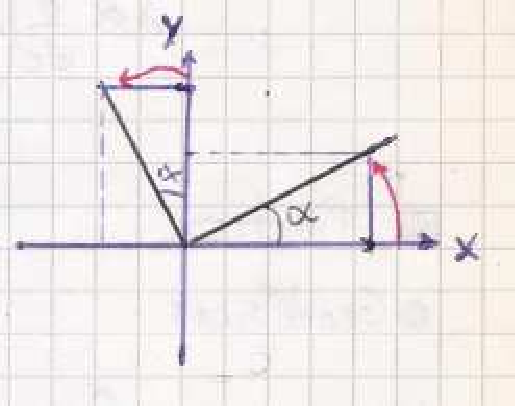
\includegraphics[width=0.35\textwidth]{images/fig_mc_noether1.pdf}	 
	\end{center}
	\caption{}
	\label{fig_mc_noether1}
\end{figure} 

Si consideramos el lagrangiano de una partícula libre en dicho plano $ \Lag = 1/2 m (\dot{x}^2 + \dot{y}^2)$, la 
cantidad conservada será 
\[
	m \dot{x} \delta x + m \dot{y} \delta y = 2\epsilon ( -p_x y + p_y x ) = cte.
\]
que no es otra cosa que el momento angular $L_z$ (que se conserva).

Por supuesto, para una rotación general (no restringida a un plano) son necesarios tres parámetros.
La rotación plana requiere solamente un parámetro.
\end{ejemplo}

% ~~~~~~~~~~~~~~~~~~~~~~~~~~~~~~~~~~~~~~~~~~~~~~~~~~~~~~~~~~~~~~~~~~~~~~

En el caso de una partícula rebotando en un billar hay simetría de rotación en torno a $z$, luego hay
constante de movimiento. En el caso del movimiento elíptico donde 1 y 2 son los focos no hay simetría
de rotación pero aún así hay constante de movimiento $ \ell_1 \ell_2 $.

\begin{figure}[!htb]
	\begin{center}
	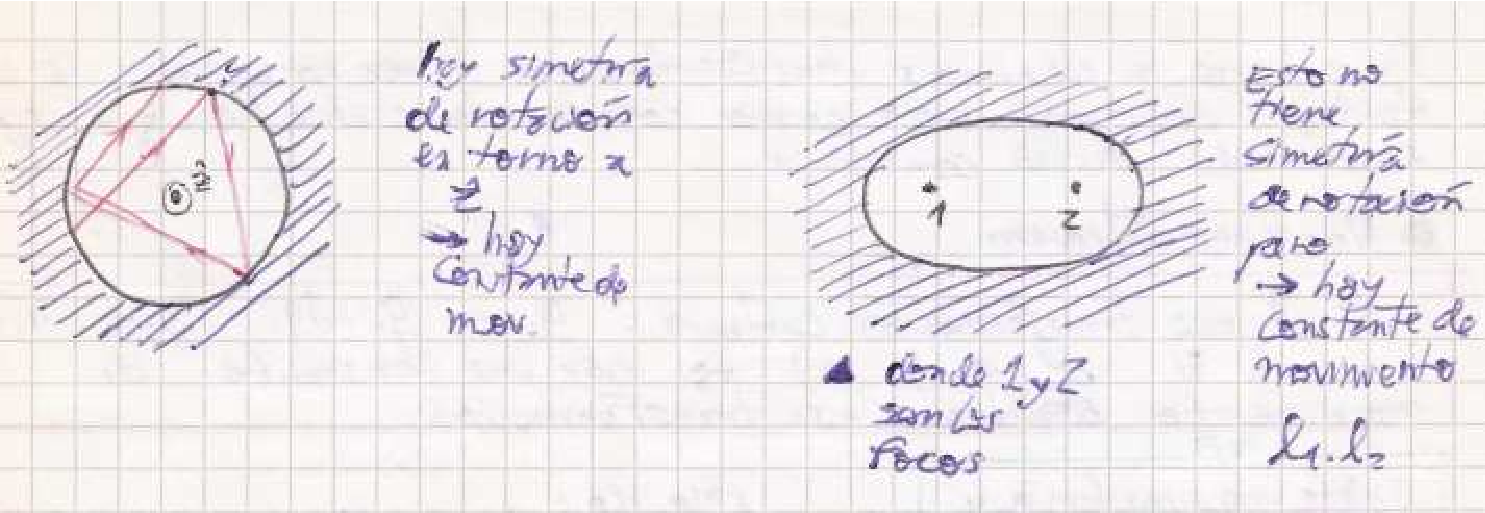
\includegraphics[width=1.0\textwidth]{images/fig_mc_noether2.pdf}	 
	\end{center}
	\caption{}
	\label{fig_mc_noether2}
\end{figure} 

\subsection{Rotación infinitesimal}

\notamargen{En la carpeta estaba este tema. Aparentemente para una rotación general aparecía el momento angular 
conservado, si se manipulaban adecuadamente los índices.}

Recordemos que 
\[
	\delta q_i = q'_i - q_i 
\]
y una traslación infinitesimal es 
\[
	\vb{r}_i' - \vb{r}_i = \delta \vb{r}. 
\]

La variable cíclica es un caso particular de teorema de Noether, pero hay constantes de movimiento que 
no provienen de ninguna simetría.
\[
	\frac{d}{dt}\left( \sum_i \dpar{\Lag}{\dot{q}_i} ( \delta \alpha \hat{n}\times \vb{r}_i ) \right) 
\]
\[
	\frac{d}{dt}\left( \delta\alpha \sum_i \vb{p}_i \times \vb{r}_i  \right) =
	\delta\alpha \frac{d}{dt}\left(  \sum_i \vb{p}_i \times \vb{r}_i  \right) = 0
\]
siendo $\delta \alpha \equiv \epsilon$ un parámetro infinitesimal.
Para $k$ grados de libertad
\begin{align*}
	q'_i &= q_i + \underbrace{\epsilon_i g_i(q_1,...,q_n,t)}_{\delta q} \\
	... \\
	q'_k &= ...
\end{align*}
\[
	\vb{r}_i' = \vb{r}_i + \delta\vb{r} \quad \textrm{traslación rígida}
\]
\[
	\vb{r}_i' = \vb{r}_i + \delta\alpha \; \hat{n}\times\vb{r}_i \quad \textrm{rotación rígida}
\]
o también 
\[
	\delta \vb{r} \times \vb{r}
\]

$T$ es invariante siempre frente a (por ser un escalar)
\[
	T = T' 
\]
entonces habrá que examinarlo.
Constatemos que 
\[
	V = V(|\vb{r}_i - \vb{r}_j|)
\]
es invariancia ante una traslación rígida, y
\[
	V = V(x_1,x_2)
\]
es una invariancia de traslación en $x_3$.

$\Lag$ tendrá como constante un momento lineal si $V$ es invariante frente a traslación.
$\Lag$ tendrá como constante un momento angular si $V$ es invariante frente a rotación.
$\Lag$ tendrá como constante una combinación si $V$ es invariante frente a una roto-traslación.

Otra construcción posible es 
\[
	\delta \Lag = 0
\]
\[
	\Lag( q_i , \dot{q}_i, t ) - \Lag(q_i' , \dot{q}_i' , t) = 0 
\]
pidiendo que $d\Lag = 0$ llego a 
\[
	\sum \left\{ \frac{d}{dt}\left( \dpar{\Lag}{\dot{q}_i} \delta q \right) - 
	\frac{d}{dt}\left( \dpar{\Lag}{\dot{q'}_i} \delta q' \right)  \right\} = 0
\]
\notamargen{Las primas están mal. Hay que pensar una construcción adecuada.
Queda odd.}
\[
	\sum \left\{ \frac{d}{dt}\left( \dpar{\Lag}{\dot{q}_i} \delta q \right) - 
	\frac{d}{dt}\left( \dpar{\Lag}{\dot{q'}_i} \delta q \right) -
	\frac{d}{dt}\left( \dpar{\Lag}{\dot{q'}_i} \sum_\ell^s \epsilon_\ell g_i^\ell \right) \right\} = 0
\]
y podemos usar que 
\[
	\dpar{\Lag}{\dot{q'}_i} = \dpar{\Lag}{\dot{q}_i}
\]
pues $g\neq g(t)$ y es todo a tiempo fijo. Se tiene 
\[
	q' = q + \delta q
\]
\[
	q_i' = q_i + \sum_\ell^s \epsilon_\ell g_i^\ell
\]
siendo esta la transformación general
\[
	\delta q_i' = \delta q_i + \sum_\ell^s \epsilon_\ell g_i^\ell
\]

Extraemos también que 
\[
	\dpar{\Lag}{\dot{q'}_i} \sum_\ell^s \epsilon_\ell g_i^\ell = C
\]

Se puede pensar también como que $\Lag$ es invariante ante la transformación infinitesimal
$\delta q$
\[
	\delta\Lag = 0 = \sum_i^N \dpar{\Lag}{q_i}\delta q_i + \dpar{\Lag}{\dot{q}_i}\delta \dot{q}_i
\]
\[
	\delta\Lag = 0 = \sum_i^N \left[ \dpar{\Lag}{q_i} - \frac{d}{dt}\left( \dpar{\Lag}{\dot{q}_i} \right)
	\right]\delta q_i  + \sum_i^N \frac{d}{dt}\left( \dpar{\Lag}{\dot{q}_i} \delta q_i \right)  = 0
\]
siendo el primer término nulo, y siendo lo que se conserva lo que aparece en el segundo término,
donde 
\[
	\delta q_i =  \sum_\ell^s \epsilon_\ell g_i^\ell(q_1,q_2,...,q_n)
\]
Finalmente 
\[
	\delta \Lag = 0 = \frac{d}{dt}\left( \sum_i^N \dpar{\Lag}{\dot{q}_i} \delta q_i \right) 
\]


% =================================================================================================


% \bibliographystyle{CBFT-apa-good}	% (uses file "apa-good.bst")
% \bibliography{CBFT.Referencias} % La base de datos bibliográfica

\end{document}
